\documentclass[tikz]{standalone}

\begin{document}
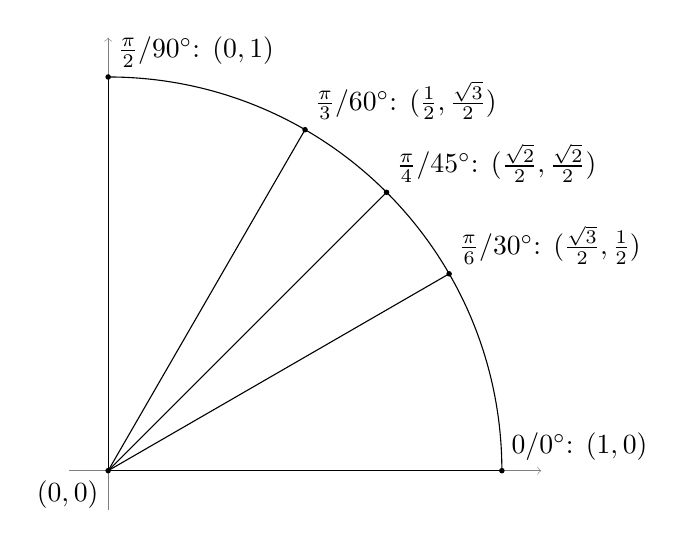
\begin{tikzpicture}[scale=5,
    point/.style={circle, inner sep=0pt, fill=black, minimum size=2pt}]
  % \draw[help lines, step=0.2] (-0.1, -0.1) grid (1.1, 1.1);
  \draw[help lines, ->] (-0.1, 0) -- (1.1, 0);
  \draw[help lines, ->] (0, -0.1) -- (0, 1.1);
  \draw (1, 0) arc [start angle=0, end angle=90, radius=1];

  \node[point] (0, 0) {};
  \node[below left] (0, 0) {$(0, 0)$};

  \draw (0, 0) -- (1, 0) node[point] {}
    node[above right] {$0$/$0^\circ$: $(1, 0)$};
  \draw (0, 0) -- (0, 1) node[point] {}
    node[above right] {$\frac{\pi}{2}$/$90^\circ$: $(0, 1)$};

  \draw (0, 0) -- (45:1) node[point] {}
    node[above right]
      {$\frac{\pi}{4}$/$45^\circ$: $(\frac{\sqrt{2}}{2}, \frac{\sqrt{2}}{2})$};

  \draw (0, 0) -- (30:1) node[point] {}
    node[above right]
      {$\frac{\pi}{6}$/$30^\circ$: $(\frac{\sqrt{3}}{2}, \frac{1}{2})$};

  \draw (0, 0) -- (60:1) node[point] {}
    node[above right]
      {$\frac{\pi}{3}$/$60^\circ$: $(\frac{1}{2}, \frac{\sqrt{3}}{2})$};
\end{tikzpicture}
\end{document}

%%% Local Variables:
%%% mode: LaTeX
%%% TeX-master: "points"
%%% End:
